\documentclass[a4paper,titlepage,twoside,12pt,leqno]{article}

\usepackage[]{fontspec}
\usepackage{xltxtra}
\usepackage[monogreek]{xgreek}

\newcommand{\en}[1]{\setlanguage{american}#1\setlanguage{monogreek}} % Για υφενώσεις στα αγγλικά

\defaultfontfeatures{Mapping=tex-text%, Scale=MatchLowercase}
} 

% Γραμματοσειρά
\setmainfont[Mapping=tex-text]{DejaVu Sans}


\usepackage{longtable} % για έναν μεγάλο πίνακα
\usepackage{graphicx, array, blindtext}

\title{Εγχειρίδιο γρήγορης αναφοράς για το ηλεκτρονικό θεματικό πάρκο σε μεσαιωνική καστροπολιτεία \\ Συχνές ερωτήσεις}
\author{Αναγνωστόπουλος Βασίλης-Θάνος, Κατσής Γιώργος}
\date{}

\begin{document}

\maketitle
\tableofcontents
\listoffigures
\listoftables
\newpage

\section{Εισαγωγή}

%Στα εγχειρίδια αυτά παρουσιάζεται η σύνταξη των εντολών με πολύ συνοπτικό τρόπο. Σε αυτά ανατρέχει ένας χρήστης ο οποίος γνωρίζει πως να χρησιμοποιεί ένα πρόγραμμα σε γενικές γραμμές αλλά δεν θυμάται τη σύνταξη κάποιας συγκεκριμένης εντολής.
\emph{Σημείωση: Τα κείμενα το οποία είναι γραμμένα σε πλάγια γραφή (όπως και το συγκεκριμένο) είναι σημειώσεις, οι οποίες θα απομακρυνθούν από το τελικό κείμενο, αλλά αυτή την στιγμή υποδηλώνουν εργασίες οι οποίες δεν μπορούν να ολοκληρωθούν χωρίς να αναπτυχθεί ο κώδικας της εφαρμογής ή για κάποιο άλλο παρεμφερή λόγο.\\}

Στο εγχειρίδιο αυτό παρουσιάζονται οι πιο συχνές ερωτήσεις πάνω στο πρόγραμμα για την αλληλεπίδραση των ενοίκων του μεσαιωνικού καστροδιαμερίσματος με τις διάφορες συσκευές και υπηρεσίες που διαθέτει το διαμέρισμα και η καστροπολιτεία.

\emph{\\Σημείωση: προτιμήθηκε η μορφή FAQ. Είναι ικανοποιητικό ή θα πρέπει να αναδομηθεί πλήρως;}

\emph{Σημείωση: Τα εγχειρίδια προτιμήθηκε να γραφούν σε λιγότερη επίσημη γλώσσα. Η επιλογή αυτή είναι λάθος;}

\section{Τί σημαίνουν τα εικονίδια στην αρχική οθόνη;}

Η πρώτη οθόνη της εφαρμογής είναι για την επιλογή του κατάλληλου μενού για την αλληλεπίδραση με την καστροπολιτεία. Στα δεξιά του παραθύρου φαίνονται σημαίες από χώρες που πατώντας και πατώντας κάποια σημαία αλλάζει η γλώσσα των μηνυμάτων που εμφανίζονται στην εφαρμογή.

Στα αριστερά της εφαρμογής φαίνονται τα εικονίδια επιλογών καθώς και ένα μικρό κείμενο το οποίο επεξηγεί τί κάνει το καθένα (βλ. σχήμα \ref{fig:menu:general})

\begin{figure}
\begin{center}
\resizebox*{10.5cm}{!}{
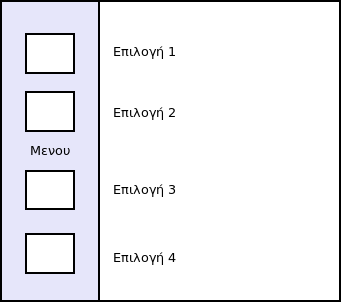
\includegraphics{images/menu.png}}
\caption{Το γενικό μενού (σε αφηρημένη μορφή).}
\label{fig:menu:general}
\end{center}
\end{figure}

Στον πίνακα \ref{table:icons} φαίνονται αναλυτικά τα εικονίδια καθώς και το τί κάνουν.

\begin{table}
\begin{center}
  \begin{tabular}{|m{0.20\textwidth}|m{0.70\textwidth}|}
    \hline
     
     \resizebox*{!}{0.20\textwidth}{
     \rule{0.4\textwidth}{0.4\textwidth}}

     & κείμενο για το σχήμα. \\ \hline



    \hline
  \end{tabular}
\caption{Τα εικονίδια της εφαρμογής}
\label{table:icons}
\end{center}
\end{table}

\emph{\\Σημείωση: Εδώ θα μπει πίνακας για να τα επεξηγεί, αλλά από την στιγμή που δεν έχει αποφασιστεί ακόμα το σχήμα τους και η λειτουργικότητα τους παραλείφθηκαν.\\}

Όταν πατηθεί κάποιο εικονίδιο τότε μεταβαίνουμε σε ένα νέο παράθυρο το οποίο αλλάζει ανάλογα με την επιλογή, όμως το μενού με τα εικονίδια στα αριστερά θα παραμένει έτσι ώστε να είναι δυνατή η εναλλαγή μεταξύ των μενού γρήγορα να είμαστε υποχρεωμένοι να γυρίσουμε στην αρχική οθόνη.


\section{Πως πραγματοποιείται μία παραγγελία στο εστιατόριο/καφετέρια;}

\emph{Μιας και δεν έχει υλοποιηθεί πλήρως το σύστημα προτιμήθηκε να μην απαντηθούν και οι υπόλοιπες ερωτήσεις, μιας και μπορούν να αλλάξουν και να αντικατασταθούν με καλύτερες. Απλώς εδώ φαίνεται ένα δείγμα για το πως θα είναι.}

\section{Πως ανοίγουμε την πόρτα του καστροδιαμερίσματος;}

\section{Πως ρυθμίζετε η θερμοκρασία στην πισίνα;}

\section{Πως ενεργοποιείται/απενεργοποιείται ο συναγερμός στην πισίνα;}


\end{document}
